\section{Конструкторский раздел}

\subsection{Требования к разрабатываемому методу}

Метод оценки безопасности водителя (далее — метод оценки) должен:
\begin{itemize}[leftmargin=1.6\parindent]
	\item[--] принимать на вход набор изображений в формате PNG, JPG, JPEG или видео в формате mp4 водителя из салона автомобиля, а также участвующие в оценке веса для каждого действия водителя, где вес -- число с плавающей точкой в диапазоне от 0 до 1;
	\item[--] в случае загрузки видео,  должен разбивать его на изображения с конфигурируемым интервалом (по умолчанию в 1 секунду);
	\item[--] выполнять предварительную обработку изображений, которые будут подаваться на вход нейронной сети;
	\item[--] вычислять оценку безопасности водителя на основе данных, полученных из обученной модели нейронной сети.
\end{itemize}

\subsection{Требования к разрабатываемому программному комплексу}
Программный комплекс, реализующий интерфейс для разработанного
метода, должен предоставлять:

\begin{itemize}[leftmargin=1.6\parindent]
	\item[--] возможность загрузить видео или набор изображений через графический интерфейс;
	\item[--] возможность задать веса для каждого действия водителя через графический интерфейс;
	\item[--] запуск вычисления оценки и ее отображение в графическом интерфейсе;
	\item[--] возможность отобразить изображения разделенные по действиям водителя в отдельном окне.
\end{itemize}

\subsection{Особенности метода оценки}
\subsubsection{Модель нейронной сети}
В качестве основы метода оценки будет использоваться модель нейронной сети GoogleNet, которая будет классифицировать изображения.

Для использования модели требуется ее предварительное обучение на размеченном наборе данных вида изображение -- класс (метка).

После обучения модель принимает изображения размером 224x224  в формате RGB  и возвращает массив вероятностей для каждого класса. Класс с наибольшей вероятностью будет считаться достоверным.

\subsubsection{Общее описание метода оценки}
Основные этапы метода оценки приведены на функциональной декомпозиции метода на рисунке  \ref{fig:idef0_A1}.

 \begin{figure}[hbtp]
	\centering
	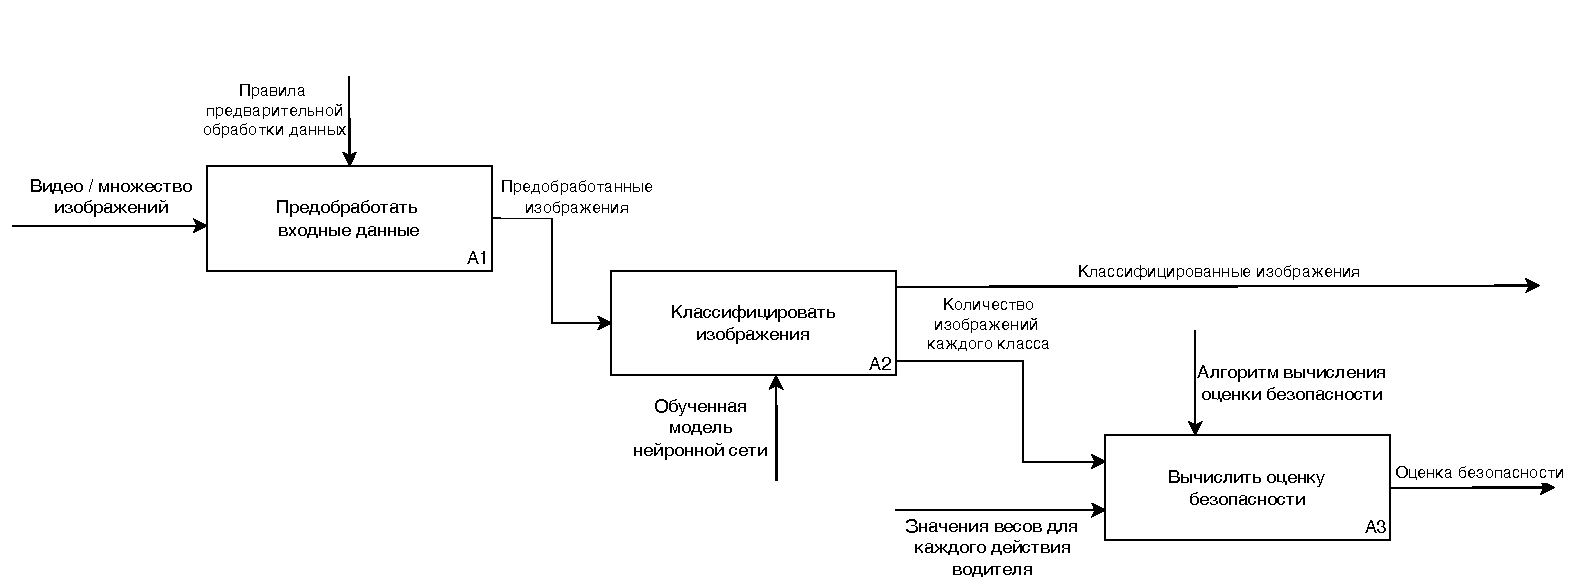
\includegraphics[width=\textwidth]{img/idef0_A1.pdf}
	\caption{Постановка задачи в виде IDEF0-диаграммы первого уровня}
	\label{fig:idef0_A1}
\end{figure}

На вход методу подается видео или множество изображений,
которые проходят предварительную обработку по определенным правилам, описанным далее.  Затем идет классификация изображений, где каждому изображению присваивается класс (метка), а также ведется подсчет количества изображений каждого класса. На основе количества изображений каждого класса  и заданных значений весов для каждого класса вычисляется оценка безопасности по алгоритму описанному далее.

\subsubsection{Предварительная обработка данных}
Разрабатываемый метод оценки предполагает предварительную обработку входных данных, схема алгоритма которой представлена на рисунке \ref{fig:prep_data}

\begin{figure}[hbtp]
	\centering
	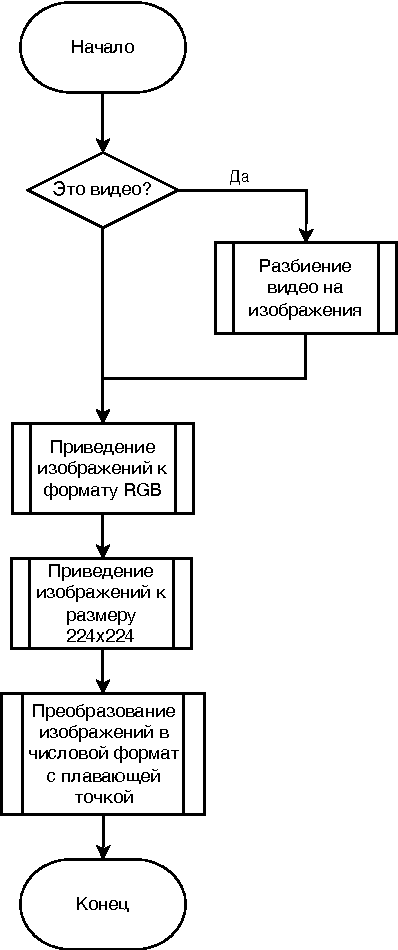
\includegraphics[scale=1]{img/prep_data.pdf}
	\caption{Схема алгоритма предварительной обработки данных}
	\label{fig:prep_data}
\end{figure}

Все перечисленные в схеме действия требуются для того, чтобы привести изображения к нужному для модели нейронной сети формату.

\subsubsection{Алгоритм вычисления оценки безопасности}
Схема алгоритма вычисления оценки безопасности на основе количества изображений каждого класса представлена на рисунке \ref{fig:assesment}.

\begin{figure}[hbtp]
	\centering
	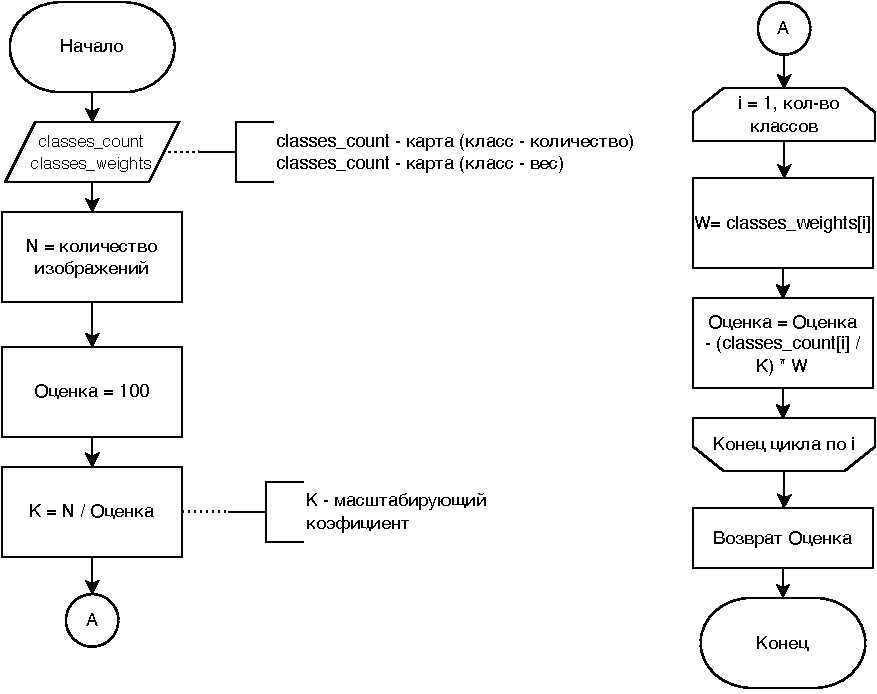
\includegraphics[scale=1]{img/assesment.pdf}
	\caption{Схема алгоритма вычисления оценки безопасности}
	\label{fig:assesment}
\end{figure}
\clearpage

\subsection{Структура разрабатываемого программного обеспечения}
Программное обеспечение состоит из четырех модулей;
\begin{itemize}[leftmargin=1.6\parindent]
	\item[--] модуль GoogleNet модели;
	\item[--] модуль пользовательского интерфейса;
	\item[--] модуль метода оценки безопасности водителя;
	\item[--] модуль загрузки и предобработки данных.
\end{itemize}


\subsubsection{Описание модулей программного комплекса}
\textbf{Модуль GoogleNet модели}

Модуль GoogleNet модели реализует модель GoogleNet для классификации изображений и предоставляет интерфейс для ее обучения.
На рисунке \ref{fig:google_net_module} представлена схема работы модуля GoogleNet модели.
\begin{figure}[hbtp]
	\centering
	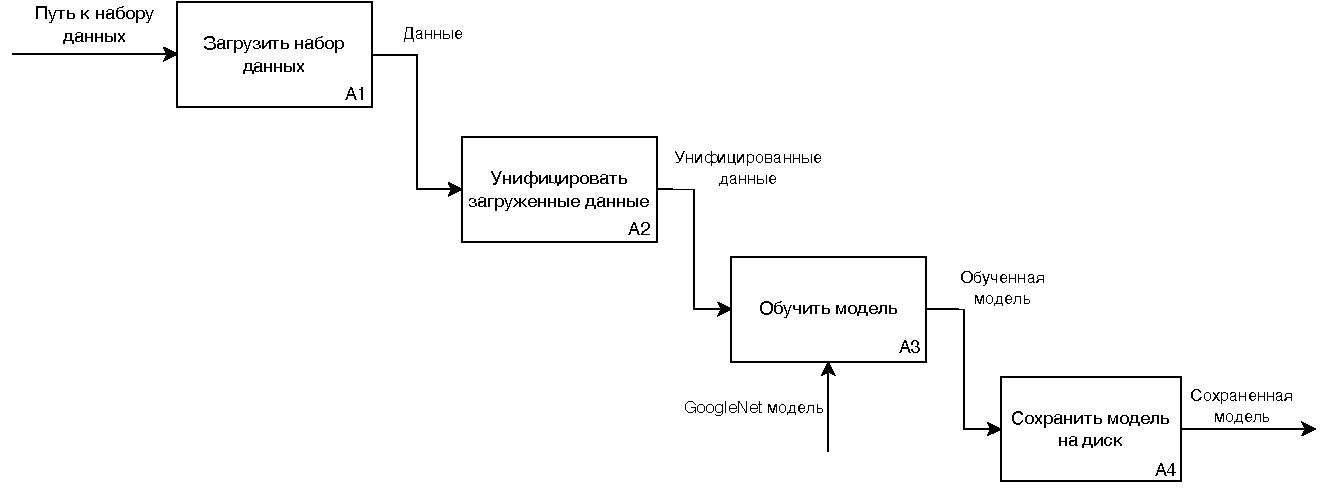
\includegraphics[scale=0.7]{img/google_net_module_v2.pdf}
	\caption{Схема работы модуля GoogleNet модели}
	\label{fig:google_net_module}
\end{figure}

В данном модуле происходит обучение модели, на тренировочном наборе данных, описанном далее. Модуль используется единожды, чтобы получить обученную модель или когда требуется внести изменения в модель. Результатом работы модуля является файл с сохраненной обученной моделью, который в дальнейшем можно загрузить и использовать как модель. Также модуль предоставляет возможность дообучать модель на каком-либо другом наборе данных.

\newpage
\textbf{Модуль пользовательского интерфейса}

Модуль пользовательского интерфейса предоставляет пользователю графический интерфейс для взаимодействия с методом оценки. Данный модуль должен давать пользователю такие возможности как: 
\begin{itemize}[leftmargin=1.6\parindent]
	\item[--] выбрать режим работы (видео или набор изображений);
	\item[--] задать путь к данным;
	\item[--] задать значения весов;
	\item[--] запустить вычисление оценки;
	\item[--] возможность просмотреть классифицированные изображения.
\end{itemize}

\textbf{Модуль метода оценки безопасности водителя}

Модуль метода оценки безопасности предоставляет программный интерфейс к методу оценки. Данный модуль загружает модель с диска, загружает данные с помощью модуля загрузки данных, предобрабатывает данные и вычисляет оценку. Результатом работы модуля являются оценка безопасности водителя и классифицированные изображения.


\textbf{Модуль загрузки  данных}

Модуль загрузки  данных предоставляет программный интерфейс позволяющий: загрузить изображения из директории,
разделить видео на изображения.


\subsubsection{Архитектура программного обеспечения}
Схема архитектуры программного обеспечения, реализующего метод оценки безопасности водителя на основе глубоких
нейронных сетей, представлена на рисунке \ref{fig:arhitectura_po}.

\begin{figure}[H]
	\centering
	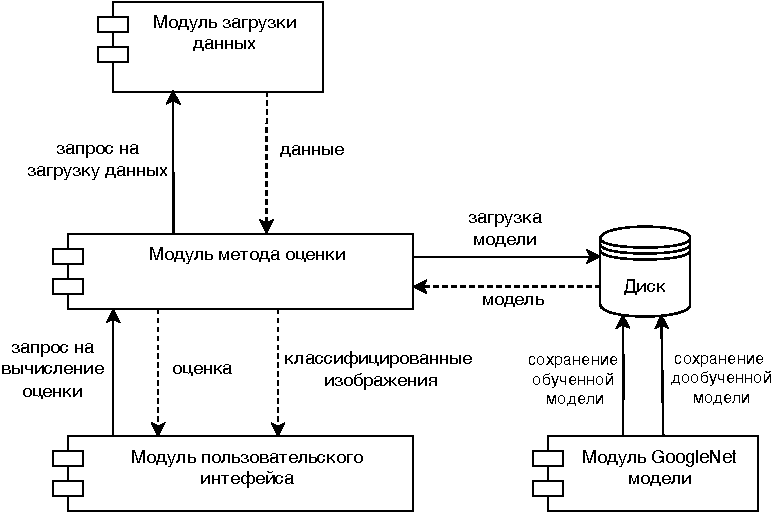
\includegraphics[scale=1.2]{img/arhitectura_po.pdf}
	\caption{Архитектура программного комплекса}
	\label{fig:arhitectura_po}
\end{figure}


\subsubsection{Данные для обучения модели}
В качестве данных для обучения модели был выбран набор данных\cite{state-farm-distracted-driver-detection}, состоящий из 22424 фотографий 26 водителей из салона автомобиля, разделенных на 10 классов:
\begin{itemize}[leftmargin=1.6\parindent]
	\item[--] сосредоточен;
	\item[--] печатает (правая рука);
	\item[--] разговаривает по телефону (правая рука);
	\item[--] печатает (левая рука);
	\item[--] разговаривает по телефону (правая рука);
	\item[--] управляет радио;
	\item[--] пьет;
	\item[--] тянется назад;
	\item[--] делает прическу/макияж;
	\item[--] разговаривает с пассажиром.
\end{itemize}

Примеры изображений для классов <<сосредоточен>> и  <<печатает (правая рука)>> представлены на рисунке \ref{fig:classes_example}.

\begin{figure}[H]
	\centering
	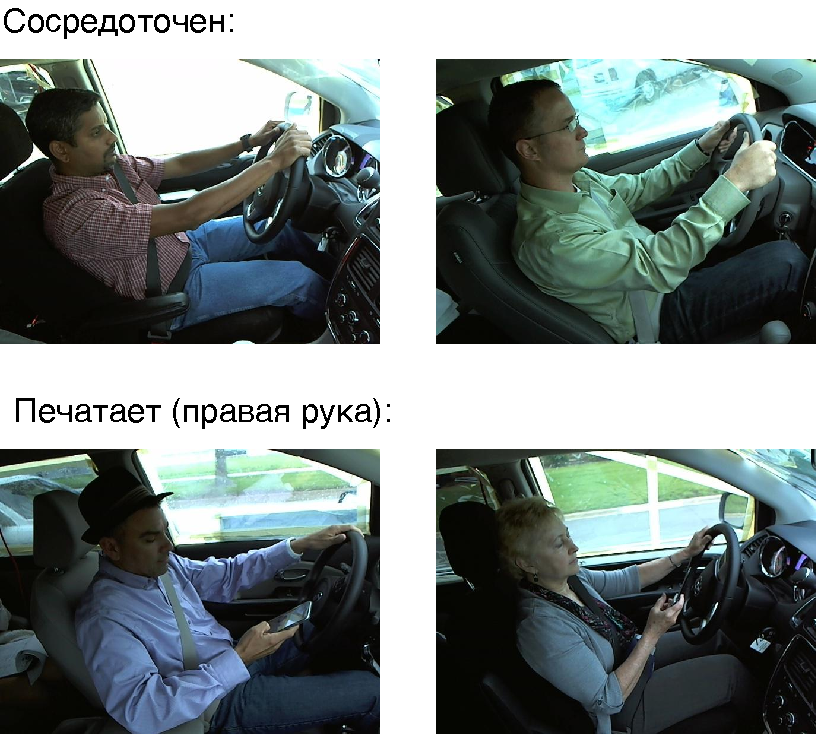
\includegraphics[scale=0.9]{img/classes_example.pdf}
	\caption{Примеры изображений из набора данных}
	\label{fig:classes_example}
\end{figure}

\subsection*{Вывод}

Были представлены требования к разрабатываемому методу оценки и программному обеспечению, реализующему интерфейс взаимодействия с методом.

Обозначены особенности разрабатываемого метода,
показано применение глубоких нейронных сетей при классификации действий водителя за рулем.

Описаны модули разрабатываемого программного обеспечения.

Представлен выбор набора данных для обучения модели и примеры из него.

\pagebreak